%\documentclass[margin=.5mm]{standalone}
%\documentclass[aspectratio=169]{beamer}
\documentclass{article}
\usepackage[legalpaper, landscape, margin=0.5in]{geometry}
\usepackage[utf8]{inputenc}
\usepackage{tikz}
\usepackage{graphicx}
\usepackage{float}
\usetikzlibrary{calc,arrows}

\usepackage{caption}
\floatstyle{plaintop}
\restylefloat{table}

\newcommand{\dittotikz}{%
    \tikz{
        \draw [line width=0.12ex] (-0.2ex,0) -- +(0,0.8ex)
            (0.2ex,0) -- +(0,0.8ex);
        \draw [line width=0.08ex] (-0.6ex,0.4ex) -- +(-1.5em,0)
            (0.6ex,0.4ex) -- +(1.5em,0);
    }%
}


\begin{document}
\begin{table}[h]
    \caption*{Horizontal Fret Movement \& Fretboard}
    \centering
    \scalebox{1.8}{
     \begin{tabular}{||c|c|c|c|c|c|c|c|c|c|c||} 
     \hline
      $4, -8$ &  $\stackrel{\rightleftharpoons}{\pm5}$ & $9, -3$  & $\stackrel{\rightleftharpoons}{\pm5}$ & $2, -10$ & $\stackrel{\rightleftharpoons}{\pm5}$ & $7, -5$ & $\stackrel{\rightleftharpoons}{\pm4}$ & $11, -1$ & $\stackrel{\rightleftharpoons}{\pm5}$ & $4, -8$  \\
     \hline \hline 
     $\odot$ & $\dittotikz$ & $5,-7$ & $\dittotikz$ & $10,-2$ & $\dittotikz$ & $3,-9$ & $\dittotikz$ & $7,-5$ & $\dittotikz$ & $0$ \\ 
     \hline \hline
     $7,-5$ &$\dittotikz$ &  $\odot$ &$\dittotikz$ & $5,-7$ &$\dittotikz$ & $10,-2$ &$\dittotikz$ & $2,-10$ &$\dittotikz$ & $7,-5$ \\ 
     \hline \hline
     $2,-10$ &$\dittotikz$ & $7,-5$ &$\dittotikz$ & $\odot$ &$\dittotikz$ & $5,-7$ &$\dittotikz$ & $9,-3$ &$\dittotikz$ & $2,-10$  \\ 
     \hline \hline
     $9,-3$ &$\dittotikz$ & $2, -10$ &$\dittotikz$ & $7,-5$ &$\dittotikz$ & $\odot$ &$\dittotikz$ & $4,-8$ &$\dittotikz$ & $9,-3$  \\
     \hline \hline 
     $5,-7$ &$\dittotikz$ & $10,-2$ &$\dittotikz$ & $3,-9$ &$\dittotikz$ & $8,-4$ &$\dittotikz$ & $\odot$ &$\dittotikz$ & $5,-7$ \\ 
     \hline \hline
     $0$ &$\dittotikz$ & $5,-7$ &$\dittotikz$ & $10,-2$ &$\dittotikz$ & $3,-9$ &$\dittotikz$ & $7,-5$ &$\dittotikz$ & $\odot$ \\ 
     \hline 
    \end{tabular}
    }
\end{table}

\vspace{6em}

\begin{figure}[h]
    \centering
    %\caption*{Fretboard}
    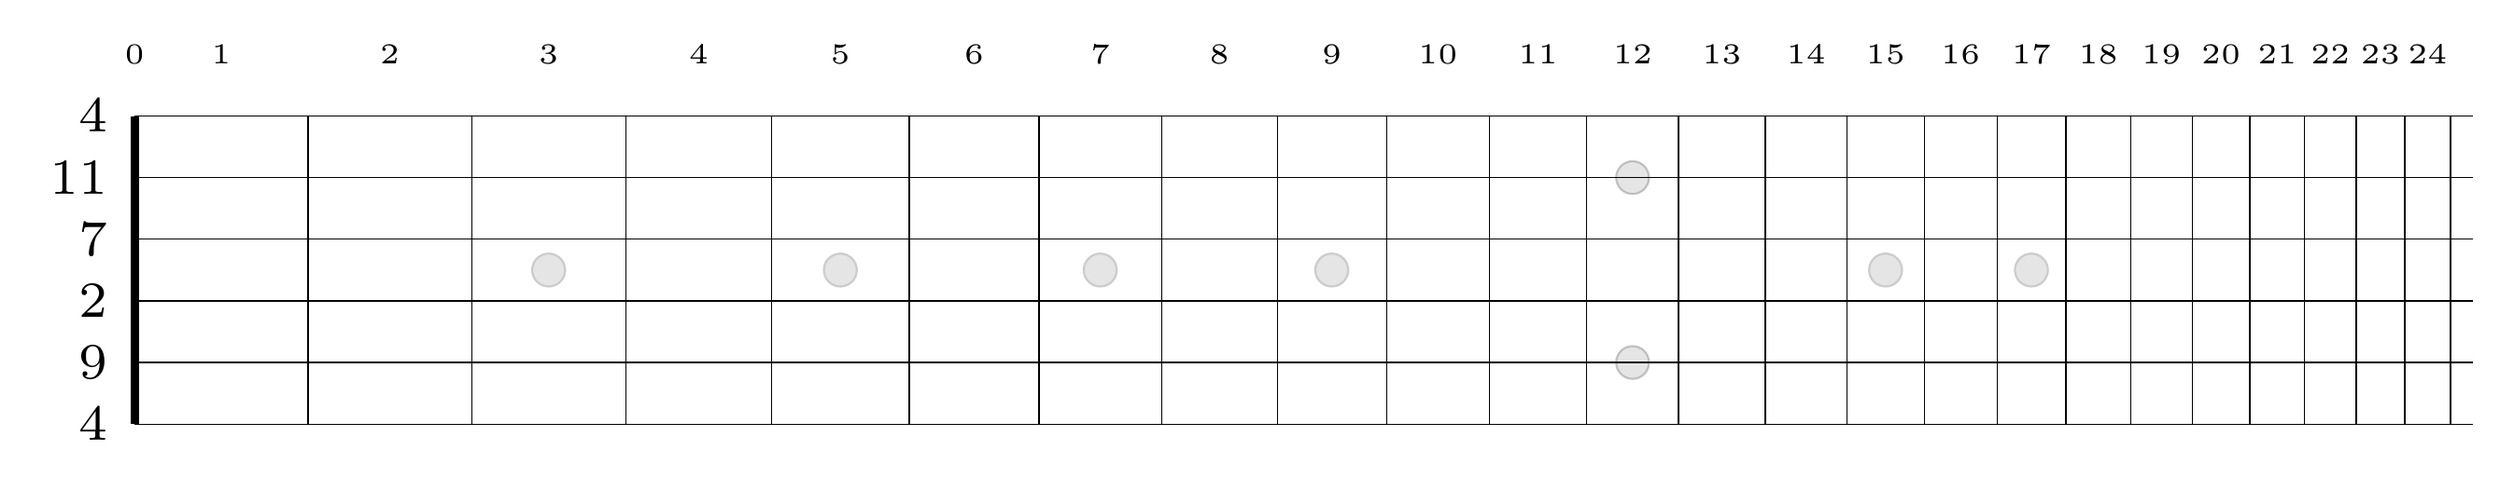
\begin{tikzpicture}[
        ynode/.style={draw=red!50,circle,fill=red!50,scale=.35,inner sep=1pt,minimum size=1.7em}, thick,scale=2.8, every node/.style={scale=2.8}]
    
      %%%% Draw the base and set coordinates %%%%
      \begin{scope}[xscale=-15,yscale=.3,line width=.5]
    
        \xdef\x{1}
        %% Left line
        \draw[line width=3] (1,1) -- (1,6);
        \foreach \fret in {1,...,24}{
          %% Set coordinate for each string
          \foreach \str in {1,...,6}{
            \coordinate (\str-\fret) at (0.97193715634*\x,\str);
          }
          %% Set coordinate for the text above
          \coordinate (Top-\fret) at (0.97193715634*\x,7);
          %% Compute the position of the fret
          \pgfmathsetmacro\x{\x * 0.94387431268}
          \xdef\x{\x}
          %% Draw the fret
          \draw (\x,1) -- (\x,6);
        }
    
        %% Draw each string
        \foreach \str in {1,...,6}{
          \draw (1,\str) -- (0.97153194115*\x,\str);
          \coordinate (start\str) at (1,\str);
        }
        \coordinate (nut) at (1,7);
      \end{scope}
    
      %% Draw the mark on the guitare
      \foreach \f in {3,5,7,9,15,17}{
        \draw[black!20,fill=black!10] ($(3-\f)!.5!(4-\f)$) circle (.08);
      }
      \draw[opacity=.20,fill,fill opacity=.10] (2-12) circle (.08) (5-12) circle (.08);
      
      
      %% DRAWS ALL THE CIRCLES ON IT %%
        %% We define the name of each number
      \newcommand\savename[2]{\expandafter\xdef\csname name#1\endcsname{#2}}
      \newcommand\getname[1]{\csname name#1\endcsname}
      \foreach \n/\t in {1/$9$,2/10,3/$11$,4/0,5/1,6/$2$,7/3,8/$4$,9/5,10/6,11/$7$,0/8}{
        \savename{\n}{\t}
      }
    
      %% Boucle on the string and the first note (given its number)
      \foreach \str/\note in {1/8,2/1,3/6,4/11,5/3,6/8}{
        \node[anchor=east] at (start\str) {\scriptsize\getname{\note}};
        %\foreach \fret in {1,...,24}{
        %  \pgfmathtruncatemacro\note{mod( \note+1, 12 )}
        %  \xdef\note{\note}
        %  \node[ynode] at (\str-\fret) {\textbf{\getname{\note}}};
        %}
      }
    
      %% Number above each space
      \foreach \fret in {1,...,24}{
        \node[scale=.8] at (Top-\fret) {\tiny \fret};
      }
    \node[scale=.8] at (nut) {\tiny 0};
    
    
    \end{tikzpicture}
\end{figure}

\newpage

\begin{table}[h]
    \caption*{Horizontal Fret Movement Explanation}
    \centering
    \scalebox{1.5}{
     \begin{tabular}{||c|c|c|c|c|c|c|c|c|c|c||} 
     \hline
      $4, -8$ &  $\stackrel{\rightleftharpoons}{\pm5}$ & $9, -3$  & $\stackrel{\rightleftharpoons}{\pm5}$ & $2, -10$ & $\stackrel{\rightleftharpoons}{\pm5}$ & $7, -5$ & $\stackrel{\rightleftharpoons}{\pm4}$ & $11, -1$ & $\stackrel{\rightleftharpoons}{\pm5}$ & $4, -8$  \\
     \hline \hline 
     $\odot$ & $\dittotikz$ & $5,-7$ & $\dittotikz$ & $10,-2$ & $\dittotikz$ & $3,-9$ & $\dittotikz$ & $7,-5$ & $\dittotikz$ & $0$ \\ 
     \hline \hline
     $7,-5$ &$\dittotikz$ &  $\odot$ &$\dittotikz$ & $5,-7$ &$\dittotikz$ & $10,-2$ &$\dittotikz$ & $2,-10$ &$\dittotikz$ & $7,-5$ \\ 
     \hline \hline
     $2,-10$ &$\dittotikz$ & $7,-5$ &$\dittotikz$ & $\odot$ &$\dittotikz$ & $5,-7$ &$\dittotikz$ & $9,-3$ &$\dittotikz$ & $2,-10$  \\ 
     \hline \hline
     $9,-3$ &$\dittotikz$ & $2, -10$ &$\dittotikz$ & $7,-5$ &$\dittotikz$ & $\odot$ &$\dittotikz$ & $4,-8$ &$\dittotikz$ & $9,-3$  \\
     \hline \hline 
     $5,-7$ &$\dittotikz$ & $10,-2$ &$\dittotikz$ & $3,-9$ &$\dittotikz$ & $8,-4$ &$\dittotikz$ & $\odot$ &$\dittotikz$ & $5,-7$ \\ 
     \hline \hline
     $0$ &$\dittotikz$ & $5,-7$ &$\dittotikz$ & $10,-2$ &$\dittotikz$ & $3,-9$ &$\dittotikz$ & $7,-5$ &$\dittotikz$ & $\odot$ \\ 
     \hline 
    \end{tabular}
    }
\end{table}


\begin{itemize}
    \item Represents the fretboard diagram rotated by $-\frac{\pi}{2}$ (clockwise rotation of $90^\circ$). In other words, a vertical guitar fretboard, as seen if it was hung up vertically.
    \item The numbers in the first row represent the pitch of the string written in Semitone Integer Notation
    \begin{itemize}
        \item The negative numbers here represent the note written in an equivalent notation, for example, the top left entry has $4, -8$ this is because a $4$ represents an $E$ in standard musical notation. This is because it is $4$ semitones above a $C$ which we write as the number $0$, additionally, if you go $8$ notes down from $C$ you also end up at an $E$.
    \end{itemize}
    \item The numbers in the rows after the first represent a jump in semitones/interval between the anchor point and some other point on the same fret, but on a different string.
    \begin{itemize}
        \item The negative numbers here have the same implication as above, in otherwords, going $x$ semitones up from any note yields the same letter name or number as going down by $x - 12$. (not considering difference in octave)
    \end{itemize}
    \item $\stackrel{\rightleftharpoons}{\pm X}$:
    \begin{itemize}
        \item  If you move from the current string and go to the string one to the right in the table (passing over $\stackrel{\rightleftharpoons}{\pm X}$ from left to right), then you add $X$ semitones 
        \item If you start on a string and go left (passing over $\stackrel{\rightleftharpoons}{\pm X}$ from right to left), you subtract $X$ semitones (notice how the notation implies this)
    \end{itemize}
    \item $\odot$ represents an anchor point, elements in the same row represent horizontal movement to the next string on the same fret. Uses for an anchor point could be a starting point to build a chord from, or just being able to move to a different location based on your most recent reference point.
    \item $\dittotikz$ represents copying whatever is in the row above to this row, it is used to reduce visual clutter
\end{itemize}


\end{document}
